\subsection{A Visual Explanation}
Proration uses two central assumptions:
\begin{itemize}
  \item The old partition and new partition have a mutual 
    refinement\footnote{in other words, they are 
    composed of the same basic building blocks.} 
    which contains population data.
  \item The voting population, and the votes for each candidate 
    are all uniformly distributed in each region of 
    the old partition.
\end{itemize}
The first assumption is almost always satisfied if the old partition 
and the new partition were drawn in the same census cycle. In this 
case, the mutual refinement is simply census blocks. The second assumption 
is problematic, but at the writing of this document, this 
is necessary in order to assign election data to the new 
partition in a reasonably fast time. At the end of this 
section are some ideas on how to bypass this assumption, and to 
assign election data in a different, more computationally 
expensive, way.

In the above example, assume that we have the following election results, 
given in old precincts:
\begin{center}
  \resizebox{0.3\textwidth}{!}{
  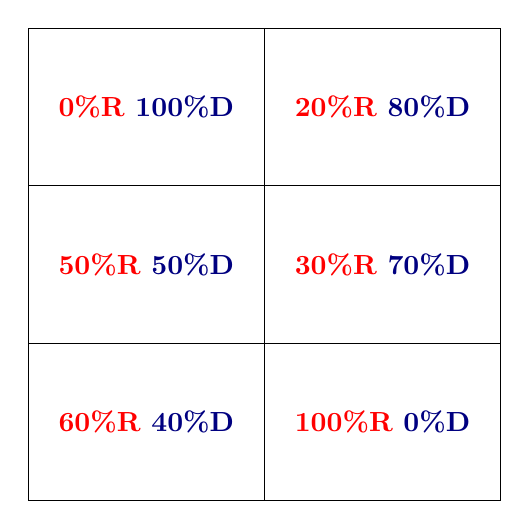
\begin{tikzpicture}
    \draw[\thicc, xstep = 3, ystep = 2] (0,0) grid (6,6);
    \node at (1.5,1) {\bf \color{Red} 60\%R \color{NavyBlue} 40\%D}; 
    \node at (4.5,1) {\bf \color{Red} 100\%R \color{NavyBlue} 0\%D};
    \node at (1.5,3) {\bf \color{Red} 50\%R \color{NavyBlue} 50\%D};
    \node at (4.5,3) {\bf \color{Red} 30\%R \color{NavyBlue} 70\%D};
    \node at (1.5,5) {\bf \color{Red} 0\%R \color{NavyBlue} 100\%D};
    \node at (4.5,5) {\bf \color{Red} 20\%R \color{NavyBlue} 80\%D};
  \end{tikzpicture}
  }
\end{center}
We take the old precincts, and the new precincts, and look at the 
pieces which constitute them - the blocks. We overlay 
the blocks on the old precincts, and use the second 
assumption to compute the election results in each block. Note 
that each block has some population, written in black.
\begin{center}
  \resizebox{0.3\textwidth}{!}{
  \begin{tikzpicture}
    \draw[\thicc, xstep = 3, ystep = 2] (0,0) grid (6,6);
    \foreach \x in {0,1,2}{
    \foreach \y in {0,1}{
    %Bottom left
    \fill[NavyBlue] (\x,\y) rectangle (\x+1,\y+.4);
    \fill[Red] (\x,\y+.4) rectangle (\x+1,\y+1);
    %Bottom right
    \fill[NavyBlue] (\x+3,\y) rectangle (\x+1,\y);
    \fill[Red] (\x+3,\y) rectangle (\x+3+1,\y+1);
    %Middle left
    \fill[NavyBlue] (\x,\y+2) rectangle (\x+1,\y+2+1/2);
    \fill[Red] (\x,\y+2+1/2) rectangle (\x+1,\y+2+1);
    %Middle right
    \fill[NavyBlue] (\x+3,\y+2) rectangle (\x+3+1,\y+2+.7);
    \fill[Red] (\x+3,\y+2+.7) rectangle (\x+3+1,\y+2+1);
    %Top left
    \fill[NavyBlue] (\x,\y+4) rectangle (\x+1,\y+4+1);
    \fill[Red] (\x,\y+4+1) rectangle (\x+1,\y+4+1);
    %Top right
    \fill[NavyBlue] (\x+3,\y+4) rectangle (\x+3+1,\y+4+.8);
    \fill[Red] (\x+3,\y+4+.8) rectangle (\x+3+1,\y+4+1);
    }
    }
    \input{fillnum.txt}
    \draw[\thicc] (0,0) grid (6,6);
    %\foreach \x in {0,...,5}{
    %\foreach \y in {0,...,5}{
    %\node at (\x+.5,\y+.5) [\thicc] {\InitVariables$\a$};
    %}
    %}
  \end{tikzpicture}
  }
\end{center}
We then multiply the vote ratios by the populations of each 
block, in order to get the vote totals in each block for each party. 
For example, below are the computed {\color{NavyBlue} \bf D} votes:
\begin{center}
  \resizebox{0.3\linewidth}{!}{
  \begin{tikzpicture}
    \draw[\thicc] (0,0) grid (6,6);
    \input{fillvotes.txt}
  \end{tikzpicture}
  }
\end{center}
Next, we overlay the new precincts, and simply add up the votes 
in order to get the new totals:
\begin{center}
  \resizebox{0.5\linewidth}{!}{
  \begin{tikzpicture}
    \draw[\thicc, Plum, xstep = 2, ystep = 3] (0,0) grid 
    (6,6);
    \input{fillvotes.txt}
    \draw [->,\thicc] (6.3,3) -- (9.7,3) node[above,midway] {Summing up};
    \draw[\thicc, Plum, xstep = 2, ystep = 3] (10,0) grid (16,6);
    \node at (1+10,1.5) {\bf \color{NavyBlue} 6.9};
    \node at (3+10,1.5) {\bf \color{NavyBlue} 4.9};
    \node at (5+10,1.5) {\bf \color{NavyBlue} 0};
    \node at (1+10,4.5) {\bf \color{NavyBlue} 6.5};
    \node at (3+10,4.5) {\bf \color{NavyBlue} 20.5};
    \node at (5+10,4.5) {\bf \color{NavyBlue} 16.1};
  \end{tikzpicture}
  }
\end{center}
Note that some of the vote totals are not integers, but are rather 
estimates of the real vote totals.
\subsection{Some psudocode}
The proration process can be also understood in terms of 
a pseudocode.
\begin{verbatim}
for i = 1 to (number of blocks):
  if block(i) is in old_precinct(j) and new_precinct(k):
    votes_in_block = (block population)*(old_precinct(j) vote percent)
    add votes_in_block to (new_precinct(k) votes)
\end{verbatim}
\subsection{Some Problems and Generalizations}
The above proration process does not work if the precincts 
do not have a good mutual refinement. In this case, there are 
a few solutions:
\begin{enumerate}
  \item The first possibility is to roundoff 
    {\it current} blocks to the {\it old} precincts, and 
    to proceed as usual. The roundoff method is explained in the 
    next section of this document.
  \item The second option is to prorate by area. This is 
    equivalent to assuming that voters are equally 
    distributed within a precinct, and then using any 
    mutual partition of the old and new precincts as a 
    base for proration (with populations added proportionally 
    to the area). 

    More concretely, in pseudocode, this is simply:
    \begin{verbatim}
for i = 1 to (number of new precincts):
  if new_precinct(i) intersects old_precinct(j):
    area(i,j) = area(new_precinct(i) intersection new_precinct(j))
    area_ratio = area(i,j)/area(old_precinct(j))
    intersection_votes = area_ratio*(old_precinct(j) vote count)
    add intersection_votes to new_precinct(i)
    \end{verbatim}
    Note that in this option, vote totals may end up as real 
    numbers, and not as pretty fractions, like in the other proration 
    methods. 
\end{enumerate}
There is also a method to do proration that is more accurate than 
anything written above, but is much more data intensive, is technically 
more involved, and requires a lot more computation power. Every 
county has a voter registration file, which in some cases has 
information on who voted in which election. These files contain the 
mailing address of every registered voter, and thus can give you a 
distribution of where voters are located within a county, and hence 
within a precinct.

Thus, using voter registration files, it might be possible to 
use vote ratios of election data in old districts to prorate 
{\it voters} instead of {\it blocks}.
